\label{sec:geometry}
\section{The Geometry of the Detector}
The IceCube detector is located at the geographic south pole in Antarctica.
The Antarctic glacier forms a 3 km deep surface of clear ice over the bedrock.
IceCube uses the Antarctic glacier as both a support structure and as a detection medium for Cherenkov radiation.

\begin{figure}
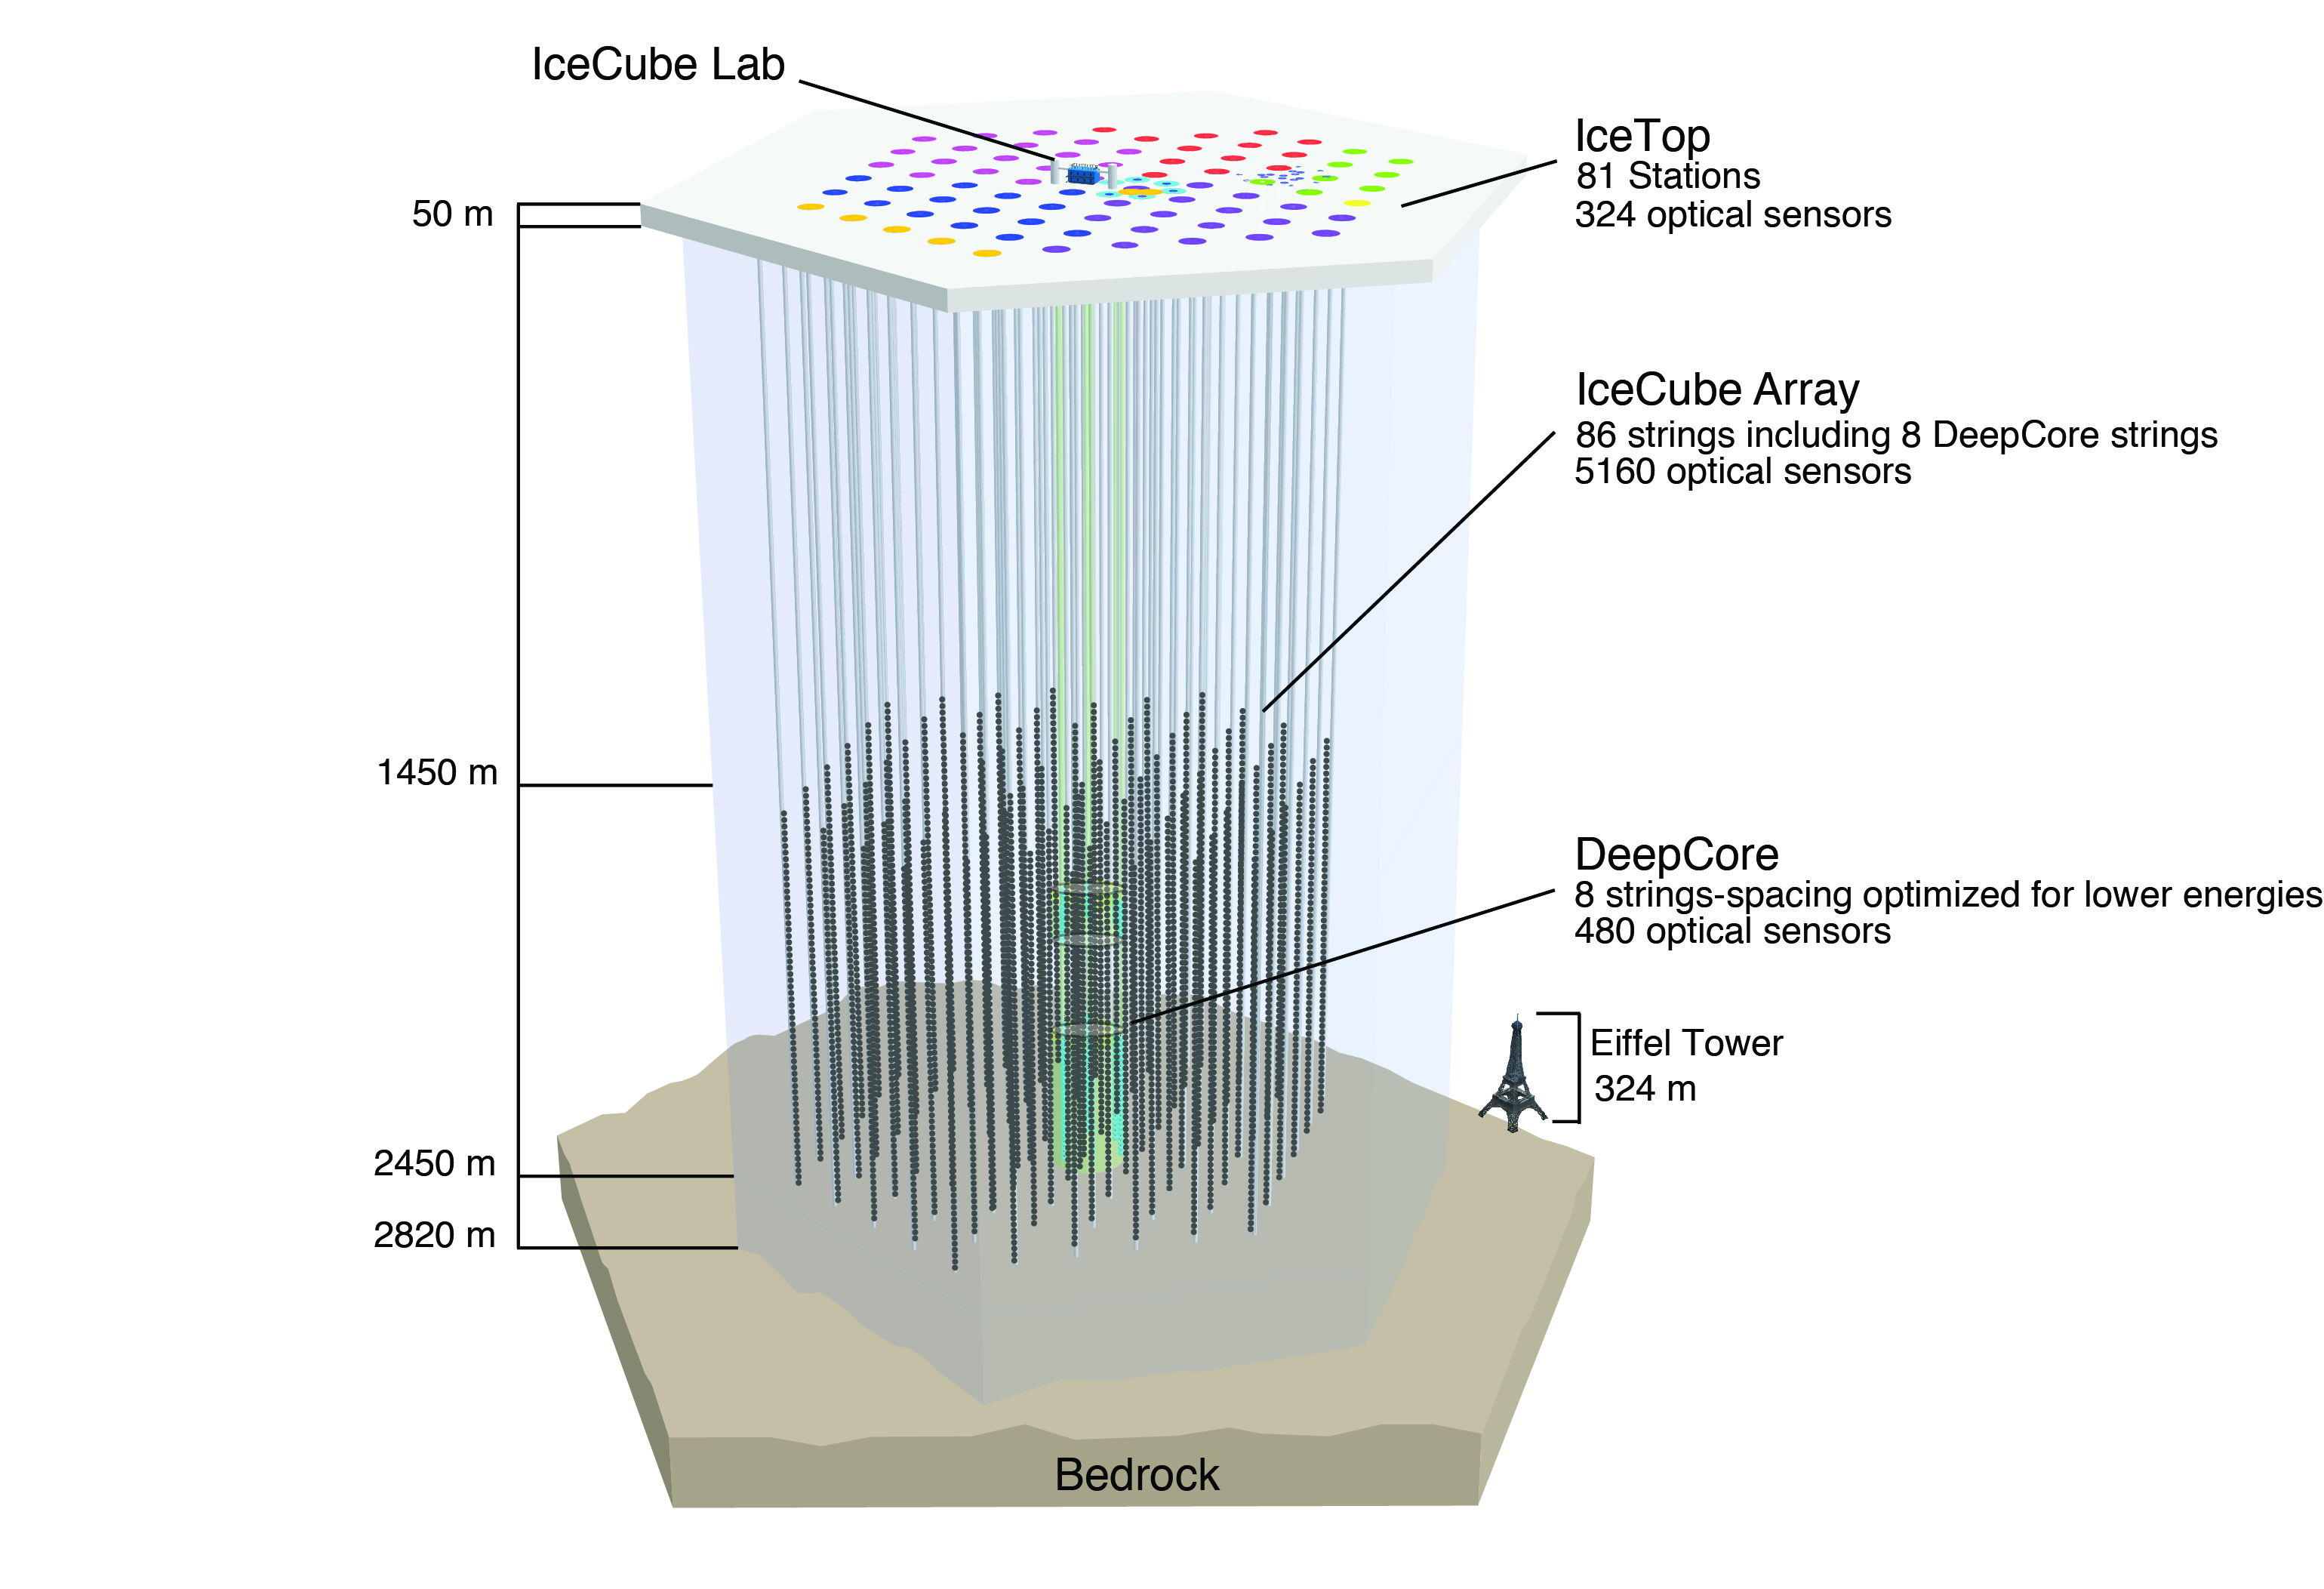
\includegraphics[width=0.9\linewidth]{ArrayWSeasonsLabels.jpg}
\caption{The IceCube Neutrino Observatory. Three separate subdetectors are shown: IceTop, a cosmic ray air shower detector; IceCube, an array designed to search for astrophysical neutrinos; and DeepCore, a dense subarray optimized for atmospheric oscillation physics measurements. The detector was deployed over multiple years. Strings deployed in the same year are shown with identical colors at the surface. }
\label{fig:icecube_depth}
\end{figure}

The IceCube observatory consists of three distinct subarrays, shown in Figure~\ref{fig:icecube_depth}, each optimized for separate physics measurements.
A total of 5160 DOMs make up the IceCube in-ice array with an additional 324 DOMs used at the surface in the IceTop air shower array \cite{Description-IceCube}.
IceCube DOMs are deployed at depths between 1450 m and 2450 m below the surface to shield the detector from atmospheric background muons.
The DOMs are deployed in a hexagonal grid in a series of 86 \emph{strings}, each of which provides connections and support for 60 DOMs.
Strings are spaced approximately 125 m apart with DOMs space 17 m apart on each string.
Each DOM in the IceCube detector is assigned a unique string number (1-86) and DOM number (1-60).

\begin{figure}
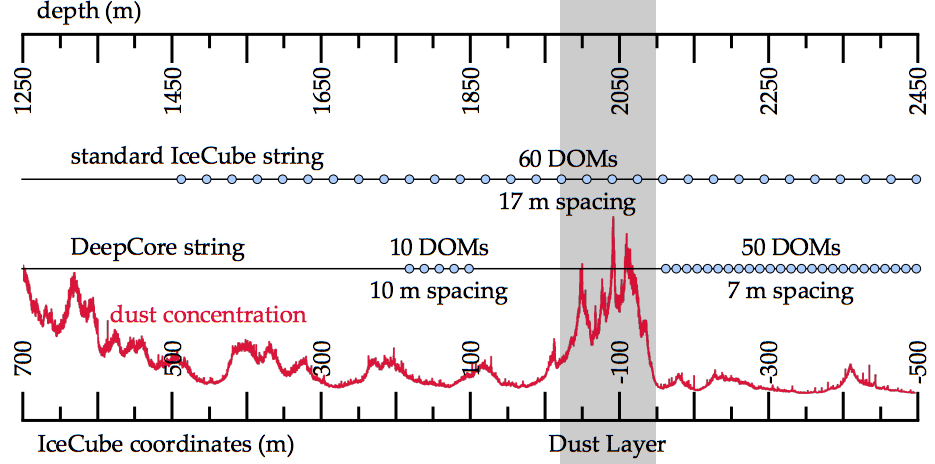
\includegraphics[width=0.9\linewidth]{icecube_depth.png}
\caption{A comparison of the standard IceCube string (right) to the DeepCore string (left). The IceCube string uses DOMs spaced 17 m apart while DeepCore divides the DOMs into a fiducial (bottom) and veto plug (top). The dust concentration is shown in red. The concentration of dust in the ice affects the scattering and absorption of the glacial ice.}
\label{fig:icecube_depth}
\end{figure}

Additional strings were installed in the glacier annually from 2004 until 2010 with partial detector data collected during construction.
During the final years of construction, a denser section of the detector was built, known as DeepCore \cite{Description-DeepCore}.
The DeepCore subarray consists of 8 strings equiped with high quantum efficiency PMTs 35\% more sensitive than the standard IceCube DOM \cite{IceCube-PMT}.
The DeepCore strings are split between a \emph{fiducial} volume, in which 50 DOMs are spaced 7 m apart on a string, and a \emph{veto plug} of 10 DOMS 10 m apart as shown in Figure~\ref{fig:icecube_depth}.
The DOMs in the DeepCore fiducial volume are located in the clearest ice of the detector at depths between 2100 m and 2450 m below the surface \cite{IceCube-SpiceMie}.
The veto cap, installed between 1750 and 1850 m below the surface, is used to identify background muons for DeepCore.

\label{subsec:icecube}
\subsection{IceCube: A Detector for TeV Neutrinos}
The IceCube detector is a regularly spaced hexagonal grid buried in the glacier with the proposed purpose of measuring astrophysical neutrino candidate events and identify the source of cosmic rays.
The IceCube array has an energy threshold of around 50-100 GeV with an optimal response above 1 TeV\cite{Description-DeepCore, Description-IceCube}.

In the standard IceCube detector, an SMT using all DOMs with a threshold of 8 HLC launches within 5 microseconds is typically used \cite{Description-IceCube}.
This trigger, known as \emph{SMT8} after the number of required hits, is designed for high signal efficiency at energies above 100 GeV with a minimum number of accidental triggers due to random detector noise.
The IceCube detector records an SMT8 rate of around 2100 Hz with less than 1 Hz expected from neutrino interactions.

Events at the TeV scales of the IceCube detector show well-defined topologies, as shown in Figure~\ref{fig:icecube_he_events}.
The IceCube detector has performed many measurements, including searches for sterile neutrinos \cite{IceCubeSterile-IC86-1}, anisotropy in the cosmic ray flux \cite{IceCube-CRAnisotropy}, measurements of the neutrino cross section at high energies \cite{IceCube-Xsec}, and the first discoveries of an astrophysical neutrino flux \cite{IceCube-HESE6}.

\begin{figure} 
\centering
    \subfloat[$\nu_e$ CC, $\nu$ NC]{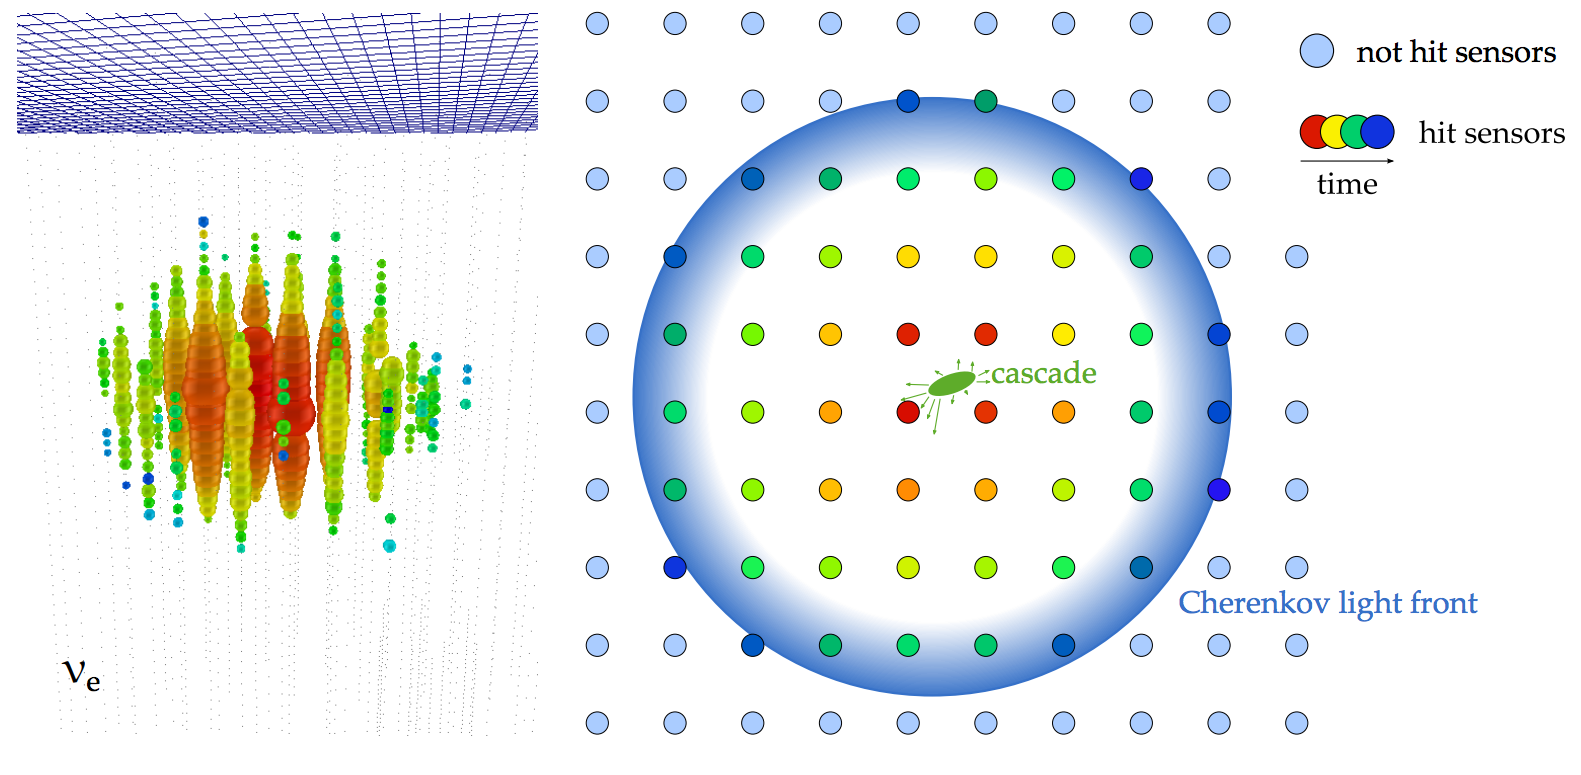
\includegraphics[width=0.7\linewidth]{icecube_he_nue.png}}
    
    \subfloat[$\nu_\mu$ CC]{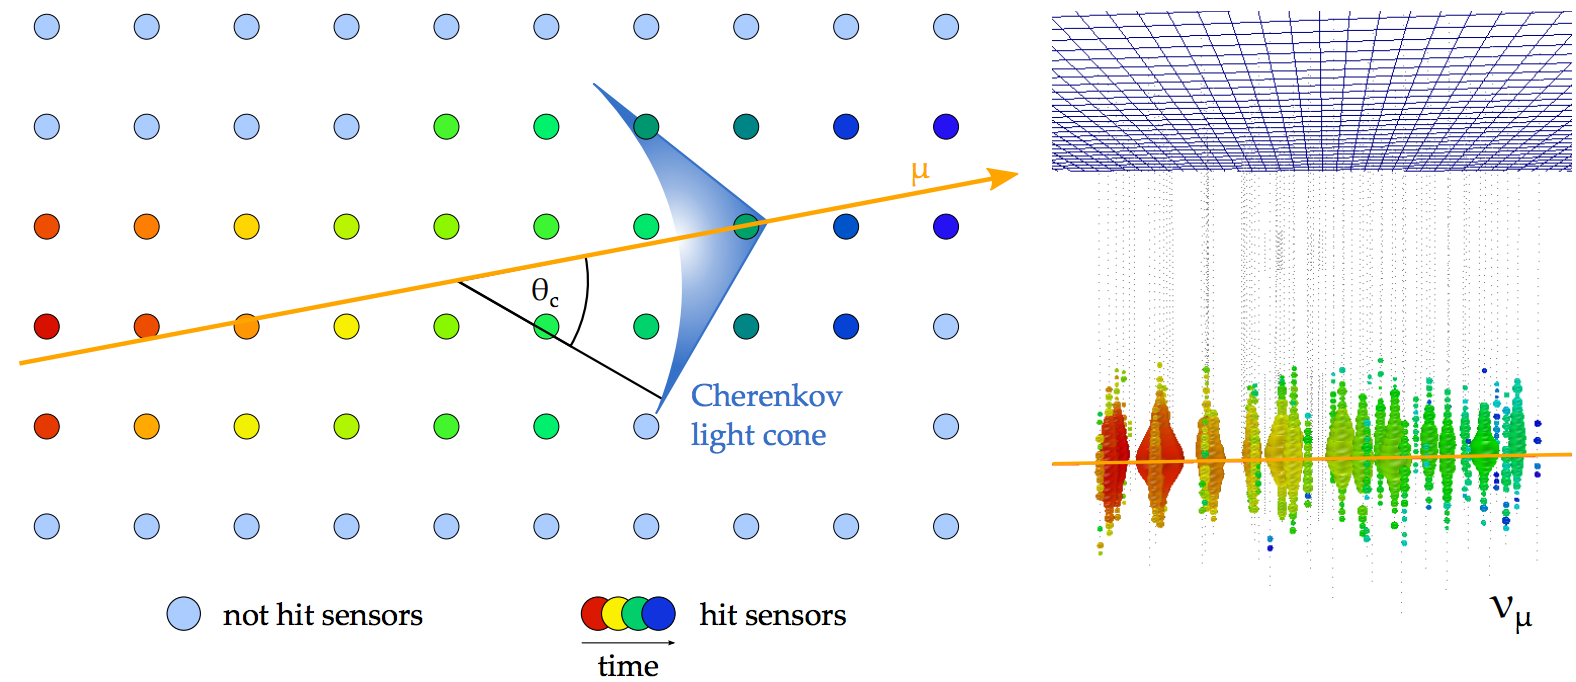
\includegraphics[width=0.7\linewidth]{icecube_he_numu.png}}
    
    \subfloat[$\nu_\tau$ CC]{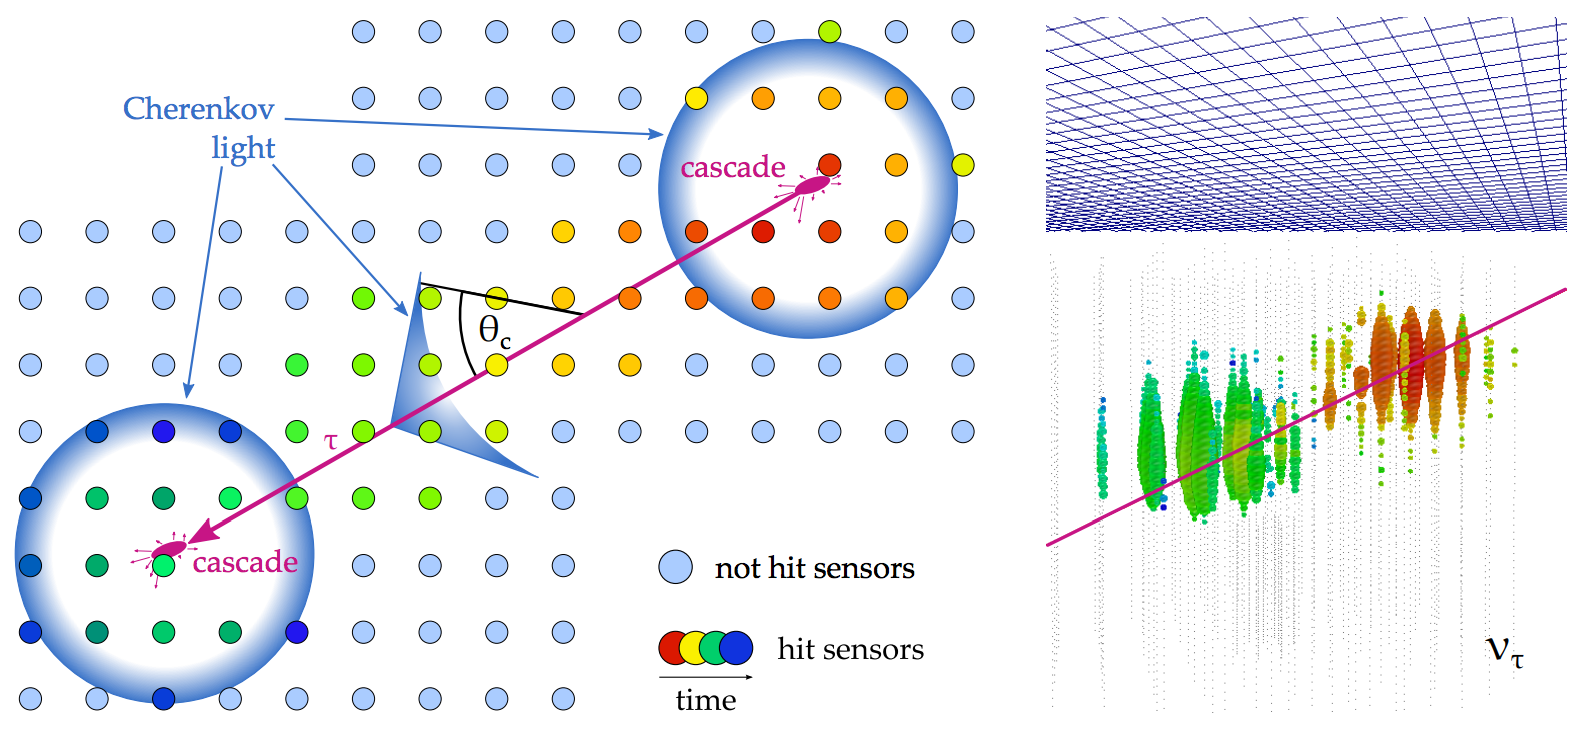
\includegraphics[width=0.7\linewidth]{icecube_he_nutau.png}} 
\caption{Examples of event topologies above 1 TeV using the full IceCube array. Event views shown in (a) and (b) are from actual events discovered by the IceCube detector \cite{IceCube-AstroNu}. Images taken from \cite{Thesis-Euler}. (a)$\nu_e$ CC and $\nu$ NC show similar behavior from electromagnetic and hadronic interactions, which result in a shower of particles that quickly scatter in the ice. Cherenkov emission from these events appears roughly spherical in the detector. These events are known as "cascades". (b) $\nu_\mu$ CC events begin with a hadronic interaction, then produce Cherenkov light from the outgoing muon. Above 1 TeV, the track of the outgoing muon becomes clearly visible. (c) Above 10 TeV, the tau lepton from a $\nu_\tau$ CC may travel a significant distance before decaying. This results in two well-separated cascades in the detector, a tell-tale signature of $\nu_\tau$ CC interactions.}
\label{fig:icecube_he_events}
\end{figure}

\label{subsec:deepcore}
\subsection{DeepCore: Extending the Reach to GeV Scales}
The DeepCore detector was designed to be a smaller, denser detector optimized for the measurement of atmospheric neutrino oscillations.
The denser spacing and clear ice of DeepCore lower the energy threshold to around 10 GeV \cite{Description-DeepCore}, permitting the study of oscillations.
DeepCore was installed at the bottom of the IceCube array near the center of the IceCube hexagonal grid, shown in Figure~\ref{fig:deepcore_layout}.

\begin{figure}
\centering
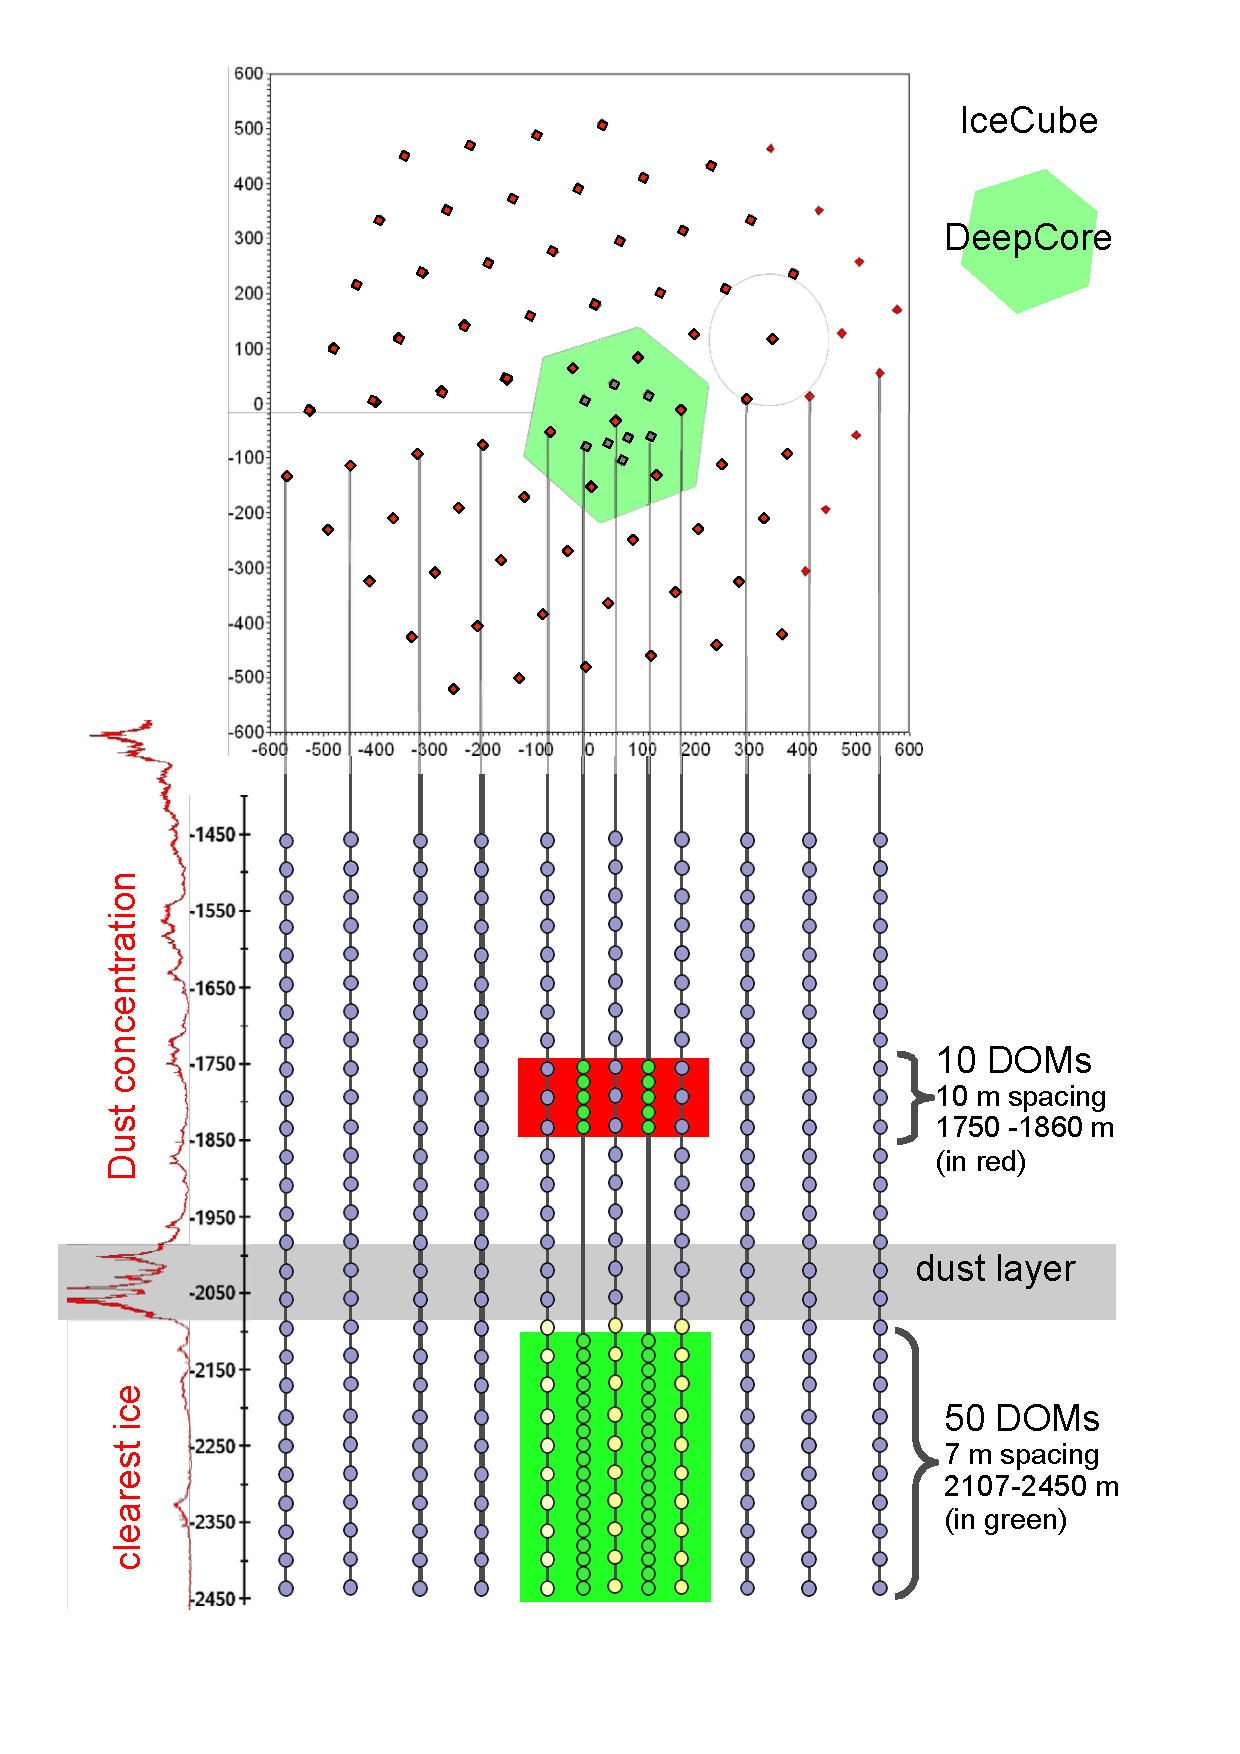
\includegraphics[width=0.6\textwidth]{dc_layout.pdf} 
\caption{The layout of the DeepCore detector. DeepCore is installed at the bottom of the IceCube detector in the clearest ice. A subset of DOMs were also deployed above DeepCore to improve muon identification of very-downgoing events.}
\label{fig:deepcore_layout}
\end{figure}

In DeepCore, the desire for lower energy events led to the introduction of a separate trigger, known as \emph{SMT3}.
This trigger, using only DOMs within the DeepCore fiducial volume, searches for at least three HLC launches occuring within 2.5 microseconds.
This effectively lowers the triggering threshold from roughly 100 GeV with the larger IceCube array to approximately 10 GeV.
The SMT3 rate, at 250 Hz \cite{Description-IceCube, Description-DeepCore}, is substantially smaller than the SMT8 rate due to both the increased overburden as well as the smaller number of PMTs included in the SMT3 DOMSet.
By placing the detector inside of the larger IceCube array, DeepCore allows analyzers to use the IceCube detector as an active veto, reducing the background rate to 17 Hz.

DeepCore events do not show the clean topological separation of the higher energy IceCube events as seen in Figure~\ref{fig:icecube_he_events}.
Events may be separated broadly into \emph{cascade-like} and \emph{track-like} statistically using information contained in the timing of hits in the detector.
Such separation techniques are energy-dependent and do not perform well at very low energies.

\begin{figure}
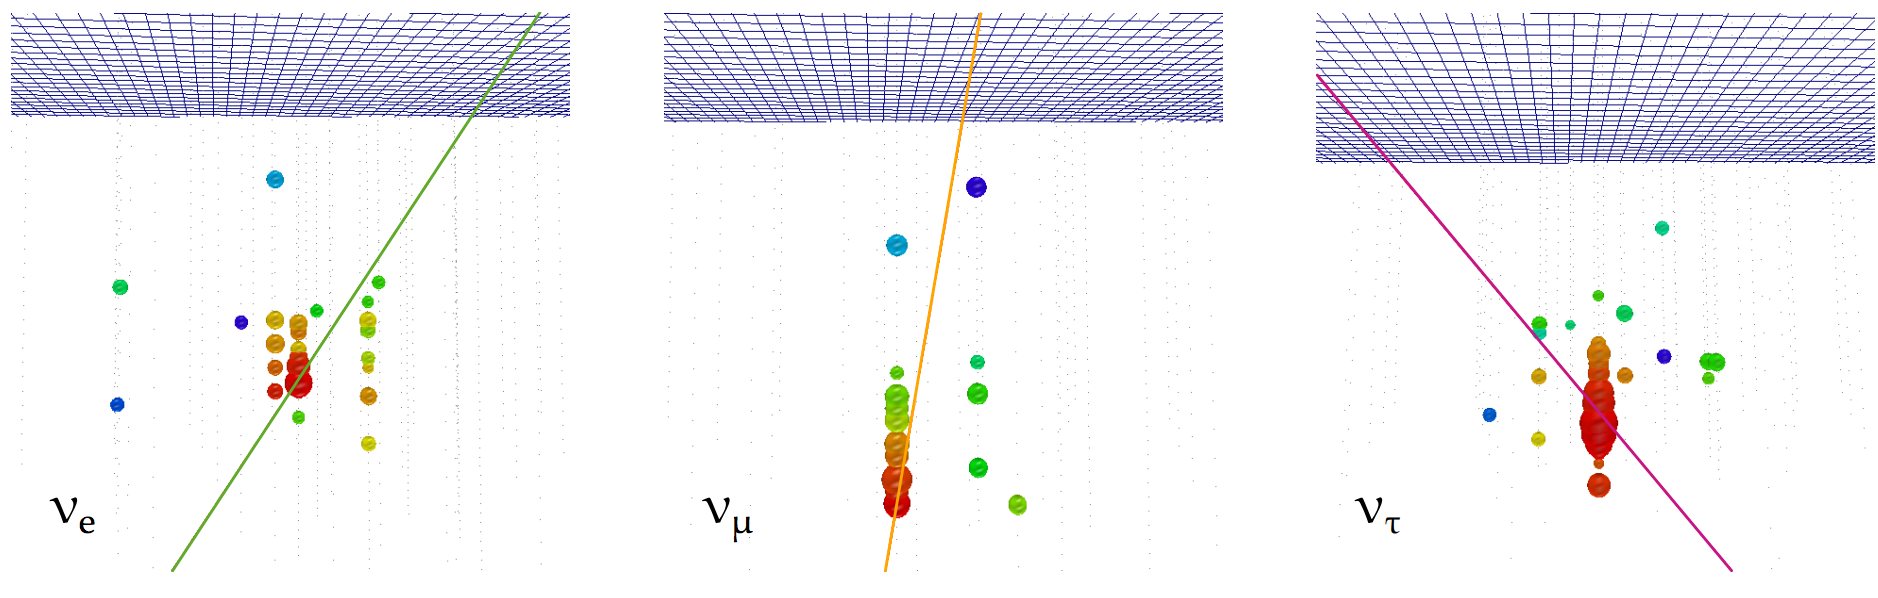
\includegraphics[width=0.9\linewidth]{deepcore_le_views.png} 
\caption{A selection of 50 GeV simulated events in DeepCore taken from \cite{Thesis-Euler}. Unlike the event topologies at high energies, DeepCore events do not show distinct event types.}
\label{fig:deepcore_events}
\end{figure}

DeepCore has observed atmospheric neutrino oscillations in the $\nu_\mu \rightarrow \nu_\tau$ in the disappearance channel \cite{IceCube-Oscillation2013,IceCube-Oscillation2015,IceCube-Oscillation2018}, with the most recent measurement showing competitive precision to dedicated measurements performed with particle accelerators.

While DeepCore was designed for oscillation physics, the neutrinos may be used for other purposes as well. 
Recent work with DeepCore has shown sensitivity to studying dark matter interactions in the sun \cite{IceCube-LE-SolarDarkMatter} and in the galaxy \cite{IceCube-LE-GalacticDarkMatter}.


